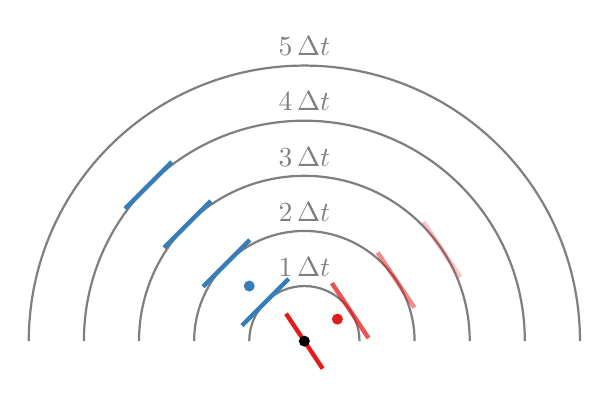
\begin{tikzpicture}[>=latex, scale=0.7]

\definecolor{Set1-3-1}{RGB}{228,26,28}
\definecolor{Set1-3-2}{RGB}{55,126,184}

\foreach \i in {1,2,3,4,5} {
  \draw[thick, opacity=0.5] (\i, 0) arc (0:180:\i);
  \node[above, opacity=0.5] at (0, \i) {$\i \, \Delta t$};
}

\fill[color=Set1-3-1] (0.6, 0.4) circle (0.1);
\begin{scope}[rotate=33.6901]
  \draw[ultra thick, Set1-3-1, opacity=1.00] (0,-0.6) -- (0, 0.6);
  \draw[ultra thick, Set1-3-1, opacity=0.75] (1,-0.6) -- (1, 0.6);
  \draw[ultra thick, Set1-3-1, opacity=0.50] (2,-0.6) -- (2, 0.6);
  \draw[ultra thick, Set1-3-1, opacity=0.25] (3,-0.6) -- (3, 0.6);
\end{scope}


\fill[Set1-3-2] (-1, 1) circle (0.1);
\begin{scope}[rotate=135]
  \foreach \i in {1,2,3,4} {
    \draw[ultra thick, Set1-3-2] (\i,-0.6) -- (\i, 0.6);
  }
\end{scope}

\fill[black] (0, 0) circle (0.1);

\end{tikzpicture}
